\section{Related Work}
\label{sec:related work}
\begin{figure*}[ht]
	\centering
	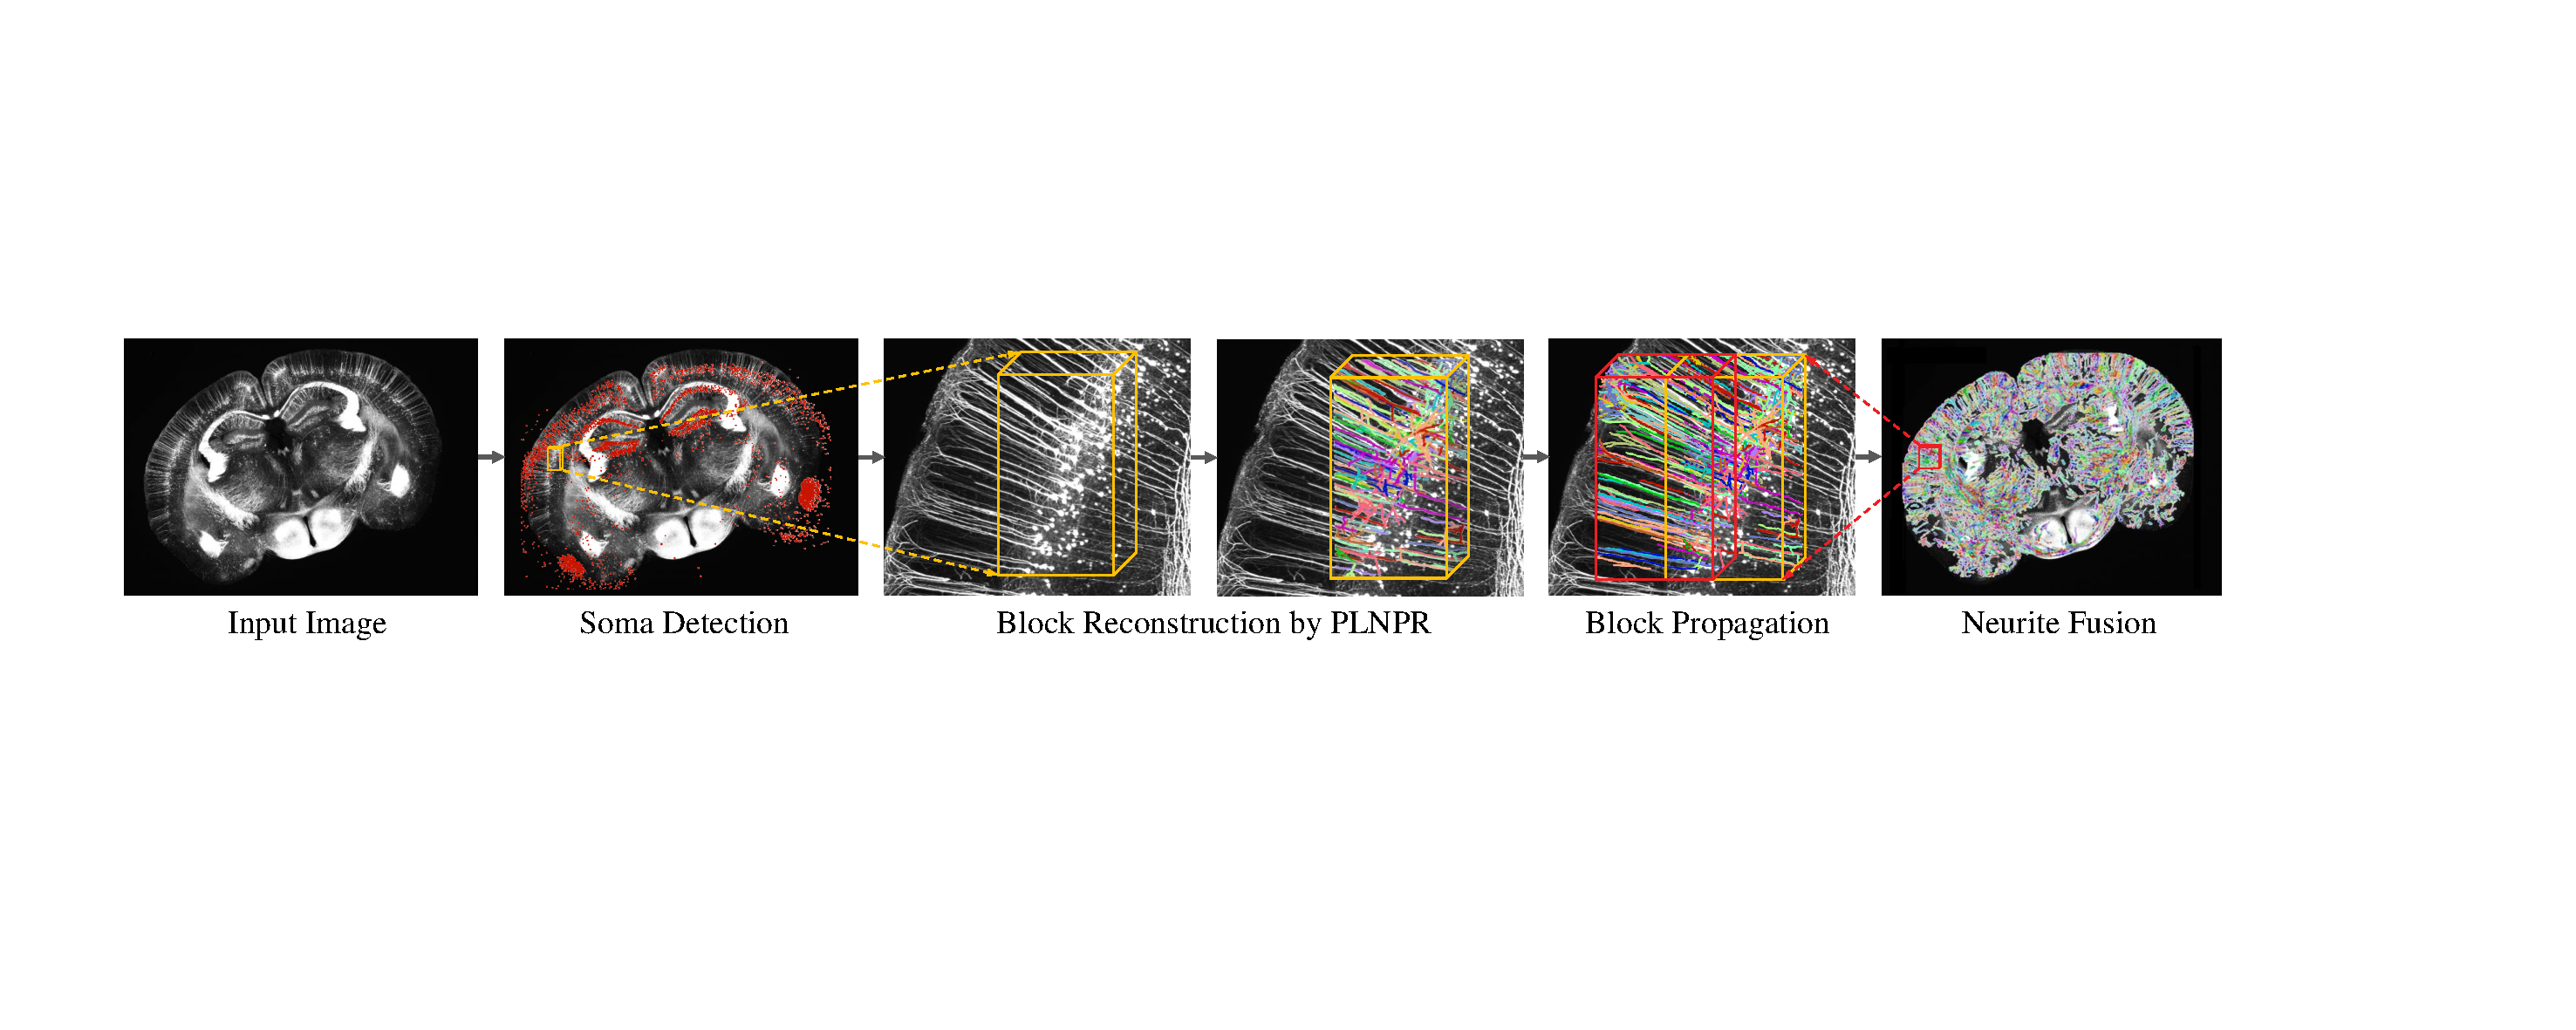
\includegraphics[width=1\textwidth]{./Illustrations/framework_ultranpr2.pdf}
	\caption{Diagram of our UltraNPR algorithm for neuronal population reconstruction from a large-scale brain slice.}
	\label{fig:ultra_framework}
\end{figure*}

%\subsection{Techniques for Robust Neuron Reconstruction}
%\label{sec:neuron reconstruction}

Early techniques for neuron reconstruction from optical microscopy images typically employ traditional image processing algorithms, such as snakes~\cite{Wang2011, Cai2006}, principal curves~\cite{Bas2011}, graph theory~\cite{Peng2010a, Yang2013, De2016}, model-fitting~\cite{Zhao2011, Santamaria2015}, watershed~\cite{Navlakha2013, Suembuel2016}, energy minimization~\cite{Quan2013, Liu2016}, mean-shift clustering~\cite{Frasconi2014}, ray-shooting~\cite{Wu2014, Liu2019}, fast-marching~\cite{Peng2011, Xiao2013, Liu2018} and so on.
Unfortunately, these conventional algorithms rely on hand-crafted features and carefully tuned parameters, and usually tend to fail when the image quality is poor.
%TReMAP~\cite{Zhou2016}, NGPST~\cite{Quan2015},

To improve the reconstruction performance from low-quality image blocks, many machine learning techniques have been introduced to extract neuron voxels from noisy and low-contrast images for further reconstruction. 
This kind of methods employs various classifiers with hand-crafted features, such as support vector machine (SVM)~\cite{Chen2015}, minimum spanning tree~\cite{Basu2016}, Bayesian probabilistic model~\cite{Radojevic2017}, Bootstrap aggregating~\cite{Wang2017}, gradient boosting decision trees (GBDT)~\cite{Gu2017}, Markov chain Monte Carlo (MCMC)~\cite{Skibbe2015, Skibbe2019}, and so on.
However, these methods employs hand-crafted features that usually suffer from limited representation capability for accurate recognition, considering more challenging and complex image blocks.


Recently, deep-learning-based methods~\cite{Li2017, Zhou2018, Xu2016,Kozinski-MIA2020} bring the power of DNNs to improve the reconstruction performance. 
Instead of manually designing sophisticated features, these DNNs learn feature representations in a data-driven way and extract more distinctive features. 
With more complicated classifiers employed to segment neuron voxels from image blocks, these methods achieve more robust reconstruction results. 
Despite great improvements, these DNN-based methods rely on extensive manual annotations of neuron voxels for network training.
Unfortunately, due to the complicated morphology of neurons and the low quality of OM images, such annotations are very costly to obtain in terms of both time and labor.
%
In comparison, we propose a novel iterative framework to progressively improve the 3D DNN-based neuron reconstruction performance without using manual annotations.


%\subsection{Large-scale Neuron Reconstruction}
%\label{sec:largescale}

%Most existing neuron reconstruction methods focus on robust and accuracy neuron reconstruction from small-size noisy image blocks. 
Despite substantial advancements brought by these methods, they often need to load all the voxels into memory.
The sheer volume of a large-scale OM image is usually far beyond the processing capability, especially on the memory cost and tracing time.
%
In recent years, some attempts have been made to reconstruct neurons from large-scale OM images, such as Neuron Crawler~\cite{Zhou2015}, UltraTracer~\cite{Peng2017} and MEIT~\cite{Wang2018}.
To tackle the challenge of huge image volume, a common solution is to reconstruct neuronal morphology block by block. 
%Each block is cropped from the raw image and is much smaller in size than the raw image.
In each local block cropped from a large-scale image, existing tracing methods, such as APP2~\cite{Xiao2013}, MOST~\cite{Wu2014} and FMST~\cite{Yang2019}, can be directly used as the base tracer to trace neurites. 
Starting from the cell body, the neurites are then traced in neighboring blocks and then fused together based on signal strengths and structure continuity.
%
However, all of these methods focus on single neuron reconstruction.
The input images usually contain only one single neuron so that the signal is very sparse without confusion of different neurons. 
%
In comparison, we target a more challenging task to reconstruct dense neuronal populations from ultra-scale OM images, where closely spaced neurites that belong to different neurons are difficult be distinguished for existing methods that are designed for single neuron reconstruction.

